\chapter{Measurements}
Several measurement campaigns were done to characterize the system.
A number of measurements were done at different solenoid tilt
angles, to estimate the effect of tilt-swing misalignment on 
the peak shifts of coils. Maps with all 21 coils
were done at a number of angles, as well as repeated measurements
for accuracy estimation. A number of procedures had to be developed
in order to make the measurements repeatable. 

\section{Fluxmeter Accuracy Estimation}
To estimate the accuracy and repeatability of the fluxmeter, 10
measurements were done under similar conditions. Coils D1-D5 as
well as Q44 were used since these have a large spread in total coil area.
The normalized standard deviation was then calculated for each coil.
Figure \ref{fig:coilarea} shows the standard deviation as a function 
of coil area.

\begin{figure}[!h]
    \centering
    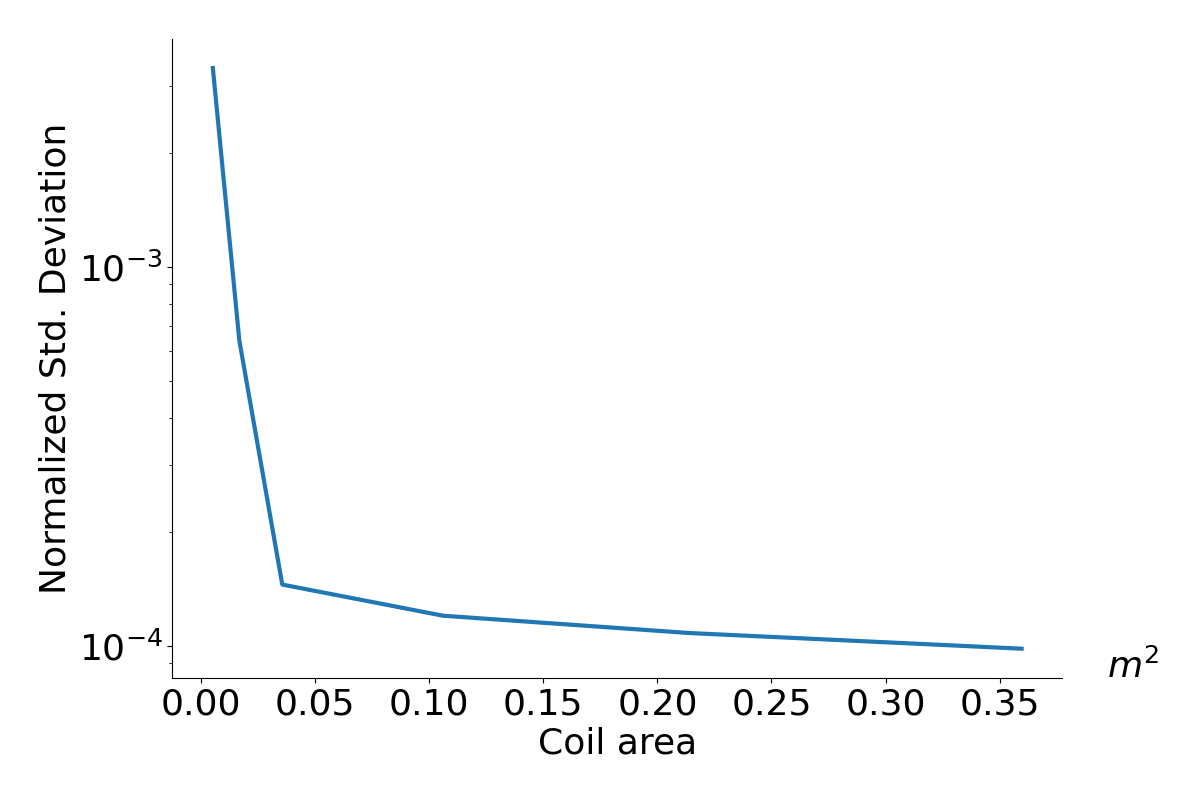
\includegraphics[width=0.8\linewidth]{figs/coilarea-error}
    \caption{Normalized measurement std. deviation as a function of
    coil area.}
    \label{fig:coilarea}
\end{figure}

As can be seen, the standard deviation of the measurements starts
increasing very fast as the coil surface area gets lower than
about $0.02$ $\text{m}^2$. A likely cause is that the signal
is starting to reach the same magnitude as the noise at this
point, which means that this is a reasonable lower bound 
on the coil surface are for a magnet of this strength ($80$ mT). 
For the region where the signal to noise ratio is high, the
standard deviation is reliably in the low promilles.

\section{The Fluxmeter Alignment Procedure}
An alignment procedure was developed for the fluxmeter, so that
measurements could be taken in an aligned, almost ideal case
or with a desired tilt angle around the $y$ axis. This will 
hereafter be referred to as the yaw angle. 

First, the laser tracker is used to sample the fluxmeter positions
as it is translated through the guiding tube. These samples are then fitted to
a line in three dimensional space, as in figure \ref{fig:geomfit}.

\begin{figure}[!h]
    \centering
    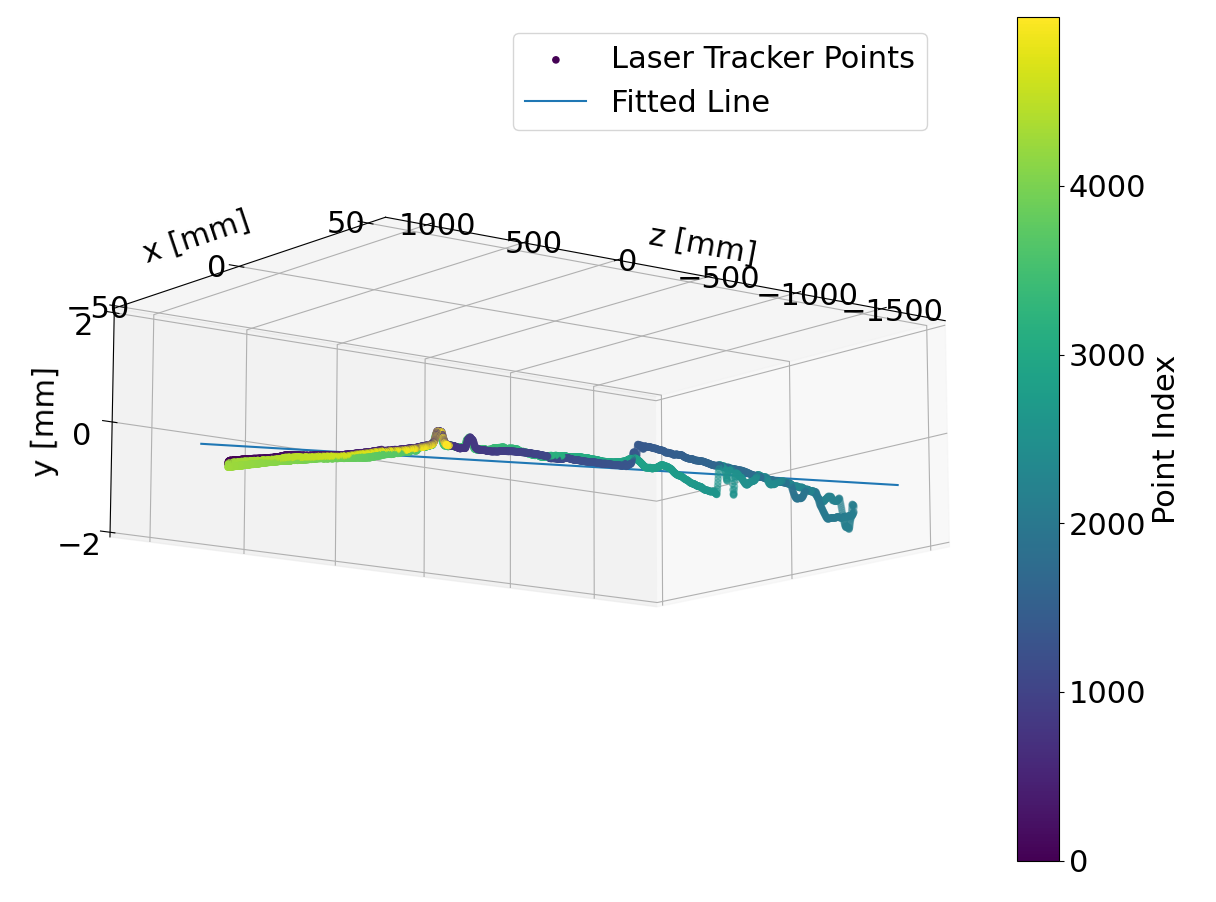
\includegraphics[width=0.8\linewidth]{figs/geomfit}
    \caption{Measured fluxmeter positions along with a line
    fit. The fluxmeter tube is tilted by $30$ mrad around the y axis.}
    \label{fig:geomfit}
\end{figure}

The intersections between the fluxmeter path line and the 
planes $z = z_{Back}$, $z = z_{Front}$ are then found, where
$z_{Back}$ and $z_{Front}$ are the $z$ offsets where the tube clamps
are located. The measured intersections $\tilde{p}_1$ and $\tilde{p}_2$
are illustrated in figure \ref{fig:alignment}.

\begin{figure}[!h]
    \centering
    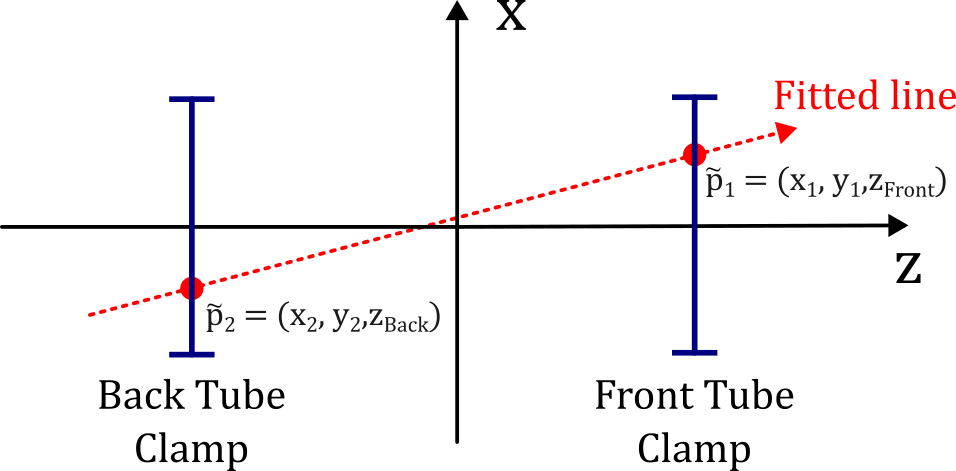
\includegraphics[width=0.8\linewidth]{figs/alignment}
    \caption{The fluxmeter path and its intersection points with
    the tube clamps.}
    \label{fig:alignment}
\end{figure}

The optimal intersect points $p_1, p_2$
are found by simple trigonometry:
\begin{align}
    p_1 = (z_{Front}\tan(\theta), 0, z_{Front}) \\ 
    p_2 = (-z_{Back}\tan(\theta), 0, z_{Back})
\end{align}
where $\theta$ is the desired yaw angle. Calculating the needed
adjustment is then a simple matter of comparing the measured
and optimal intersect points. The front clamp is adjusted by
$\tilde{p}_1 - p_1$ and the back clamp by $\tilde{p}_2 - p_2$.

The fluxmeter path is then measured again with the laser tracker,
and the whole procedure is iterated until the desired yaw angle
is reached, to an accuracy of 
$|\tilde{p}_1 - p_1|, |\tilde{p}_2 - p_2| < 0.2$ mm.
$z_{Front} - z_{Back} = 1521$ mm, making the yaw angle error
less than $0.26$ mrad.

\section{Peak Shift Measurements}
In section \ref{}